\documentclass{standalone}

%----------------------------------------------------------------------------------------------%
%                                 Packages and basic declarations
%----------------------------------------------------------------------------------------------%

\usepackage[utf8]{inputenc}
\usepackage{pgfplots}
\usepackage{tikz}
\usepackage{nicefrac}


%----------------------------------------------------------------------------------------------%
%----------------------------------------------------------------------------------------------%
%                                            DOCUMENT STARTS
%----------------------------------------------------------------------------------------------%
%----------------------------------------------------------------------------------------------%

\begin{document}


%Tikz picture starts%

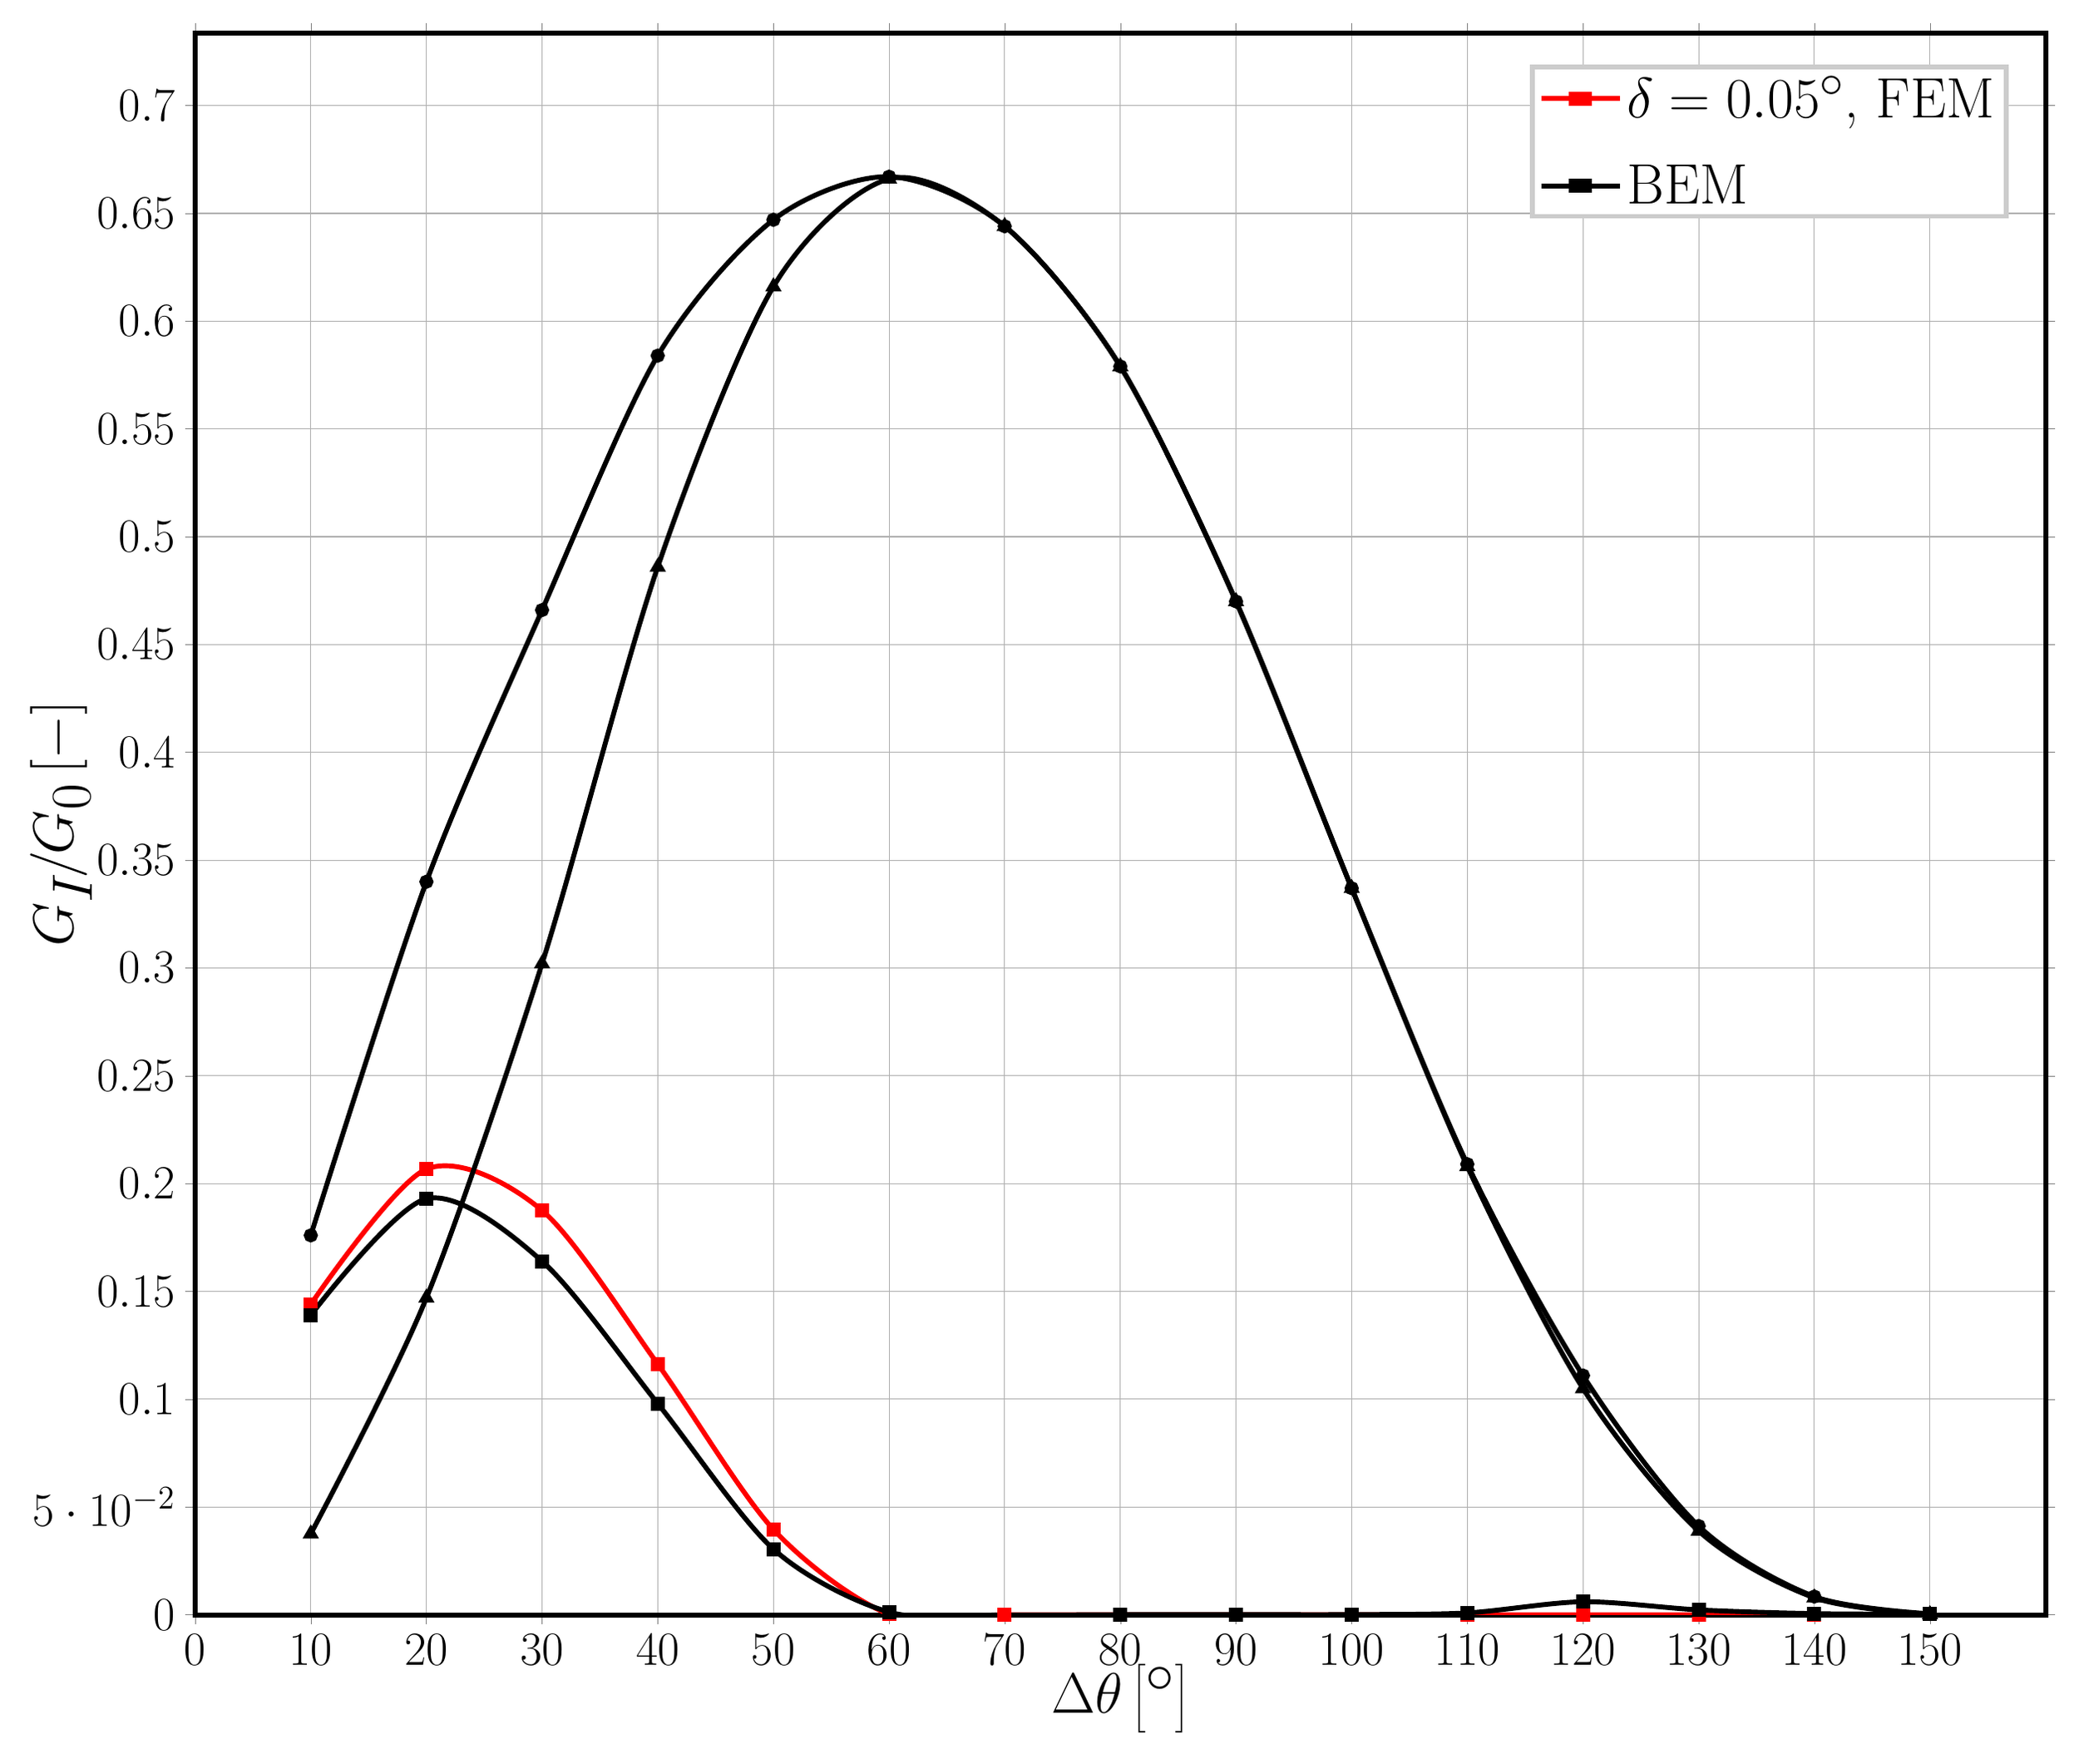
\begin{tikzpicture}

%Tikz axis starts%

\begin{axis}[width=30cm,
% STYLE
%title style={font=\fontsize{40}{8}\selectfont},
xlabel style={at={(axis description cs:0.5,-0.025)},anchor=north,font=\fontsize{48}{40}\selectfont},
ylabel style={at={(axis description cs:-0.05,.5)},anchor=south,font=\fontsize{48}{40}\selectfont},
tick align=outside,
tick label style={font=\huge},
legend style={draw=white!80.0!black,font=\fontsize{28}{24}\selectfont,row sep=15pt},
legend image post style={xscale=2},
legend cell align={left},
% GRID STYLE
xmajorgrids,
x grid style={lightgray!92.026143790849673!black},
ymajorgrids,
y grid style={lightgray!92.026143790849673!black},
line width=0.75mm,
% GRID SIZE
xmin=0.0,
xmax=160.0,
ymin=0.0,
xtick={0.0,10.0,20.0,30.0,40.0,50.0,60.0,70.0,80.0,90.0,100.0,110.0,120.0,130.0,140.0,150.0},
% CONTENT
%title={\bf{$\frac{G_{I}}{G_{0}}$ as function of debond's size $\Delta\theta$, in-house VCCT routine}},
xlabel={$\Delta\theta\left[^{\circ}\right]$},
ylabel={$\nicefrac{G_{I}}{G_{0}}\left[-\right]$},
% LEGEND ENTRIES
legend entries={{$\delta=0.05^{\circ}$, FEM},{BEM}},
]

% ==========>  GI

% =====> FEM 0.05°

\addplot[red,smooth,mark=square*]
table{
10.0	 0.143990
20.0	 0.206722
30.0	 0.187559
40.0	 0.116317
50.0	 0.039612
60.0	 0.000335
70.0	 0.000008
80.0	 0.000012
90.0	 0.000011
100.0 0.000010
110.0 0.000006
120.0 0.000004
130.0 0.000001
140.0 0.000000
150.0 0.000444
};


% ==========> BEM

%GI
\addplot[black,smooth,mark=square*]
table{
10.0   0.139
20.0   0.193
30.0   0.164
40.0   0.098
50.0   0.0305
60.0   0.00127
70.0   -4.79e-05
80.0   6.85e-05
90.0   0.000112
100.0 0.000112
110.0 0.000895
120.0 0.00607
130.0 0.00229
140.0 0.000552
150.0 0.000306
};

%GII
\addplot[black,smooth,mark=triangle*]
table{
10.0	0.037600
20.0	0.147000
30.0	0.302000
40.0	0.486000
50.0	0.616000
60.0	0.666000
70.0	0.644000
80.0	0.579000
90.0	0.470000
100.0	0.337000
110.0	0.208000
120.0	0.105000
130.0	0.038900
140.0	0.007920
150.0	0.000165
};

%GTOT
\addplot[black,smooth,mark=*]
table{
10.0	0.176000
20.0	0.340000
30.0	0.466000
40.0	0.584000
50.0	0.647000
60.0	0.667000
70.0	0.644000
80.0	0.579000
90.0	0.470000
100.0	0.337000
110.0	0.209000
120.0	0.111000
130.0	0.041200
140.0	0.008470
150.0	0.000471

};

\end{axis}
%Tikz axis ends%


\end{tikzpicture}
%Tikz picture ends%


\end{document}

%----------------------------------------------------------------------------------------------%
%----------------------------------------------------------------------------------------------%
%                                            DOCUMENT ENDS
%----------------------------------------------------------------------------------------------%
%----------------------------------------------------------------------------------------------%
